\section{Introduction}

Knowledge distillation transfers knowledge from a strong teacher to a weaker student and is particularly valuable for compact language models~\citep{hinton2015distilling,gu2024minillm,pmlr-v235-ko24c}. On-policy distillation (OPD) applies this paradigm to student-generated responses, providing dense teacher guidance on the student's own generation distribution~\citep{agarwal2024policy}. For each sampled token, OPD derives an advantage from the difference between its teacher and student log-probabilities. This dense signal underlies strong recent OPD methods~\citep{yang2026learning,li2026filter,zhao2026poweropd}, but measures teacher preference rather than verified task success.

This distinction is particularly important for long-context tasks, where correct responses must integrate evidence scattered across distant positions and satisfy global task constraints~\citep{bai2024longbench,hsieh2024ruler,goldman2024really,bai2025longbench}. With longer inputs, student models are more likely to produce locally plausible but globally incomplete responses, as they can struggle to locate and use relevant information when its position or lexical form changes~\citep{liu2024lost,pmlr-v267-modarressi25a}. A response may therefore receive strong teacher support while omitting required evidence. Task-specific verifiers, in contrast, evaluate task completion at the response level and may return graded rewards that reflect partial success~\citep{shao2024deepseekmath}. We call discrepancies between teacher preference and verified task outcomes teacher--verifier disagreement. Figure~\ref{fig:teacher-verifier-motivation} presents diagnostic evidence from a fixed set of generated responses in two representative tasks that share this evidence-aggregation requirement. In both, trajectory-level OPD scores become progressively less aligned with verifier rewards across the analyzed input-length ranges. This trend motivates an interface that preserves dense teacher guidance while correcting response-level preferences inconsistent with verified outcomes.

Existing verifier-aware OPD methods use outcome feedback through objective routing, teacher-context reconstruction, outcome-class calibration, or token-level gating~\citep{zheng2026scope,yu2026multi,hou2026uni,xu2026sg}. These methods establish that verifier feedback complements dense teacher guidance. However, they do not simultaneously preserve graded within-group outcome differences and translate the resulting response-level discrepancy into token-dependent calibration while retaining the original OPD advantage.

To address these limitations, we propose Group-Calibrated On-Policy Distillation (GC-OPD). Following the group-relative comparison in Group Relative Policy Optimization~\citep{shao2024deepseekmath}, GC-OPD separately normalizes verifier rewards and trajectory-level OPD scores within each rollout group. As Figure~\ref{fig:gcopd-overview} shows, their difference forms a signed residual whose direction and magnitude quantify teacher--verifier disagreement. Subtracting the group-normalized OPD assessment focuses calibration on their discrepancy rather than directly adding verifier feedback. Relative-advantage-based credit assignment (RACA) distributes this residual across tokens according to their relative OPD advantages while retaining the original dense OPD signal.

Our contributions are as follows:
\begin{itemize}
    \item We identify a shared pattern across two distributed-evidence long-context tasks: trajectory-level OPD scores become progressively less aligned with verifier rewards over longer inputs, as measured by pairwise disagreement rate and OPD preference gap.
    \item We propose GC-OPD, which retains the original OPD advantage while forming a signed residual between group-normalized verifier rewards and trajectory-level OPD scores. RACA distributes this residual across tokens using relative OPD advantages.
    \item Across two model scales and five long-context benchmarks, GC-OPD achieves the highest average score under the shared setup. Ablations show that the signed residual is more effective than either an additional OPD-derived term or direct group-normalized verifier reward addition, while RACA improves over uniform token allocation.
\end{itemize}

\ifdefined\GCOPDSingleColumnLayout
\begin{figure}[t]
\centering
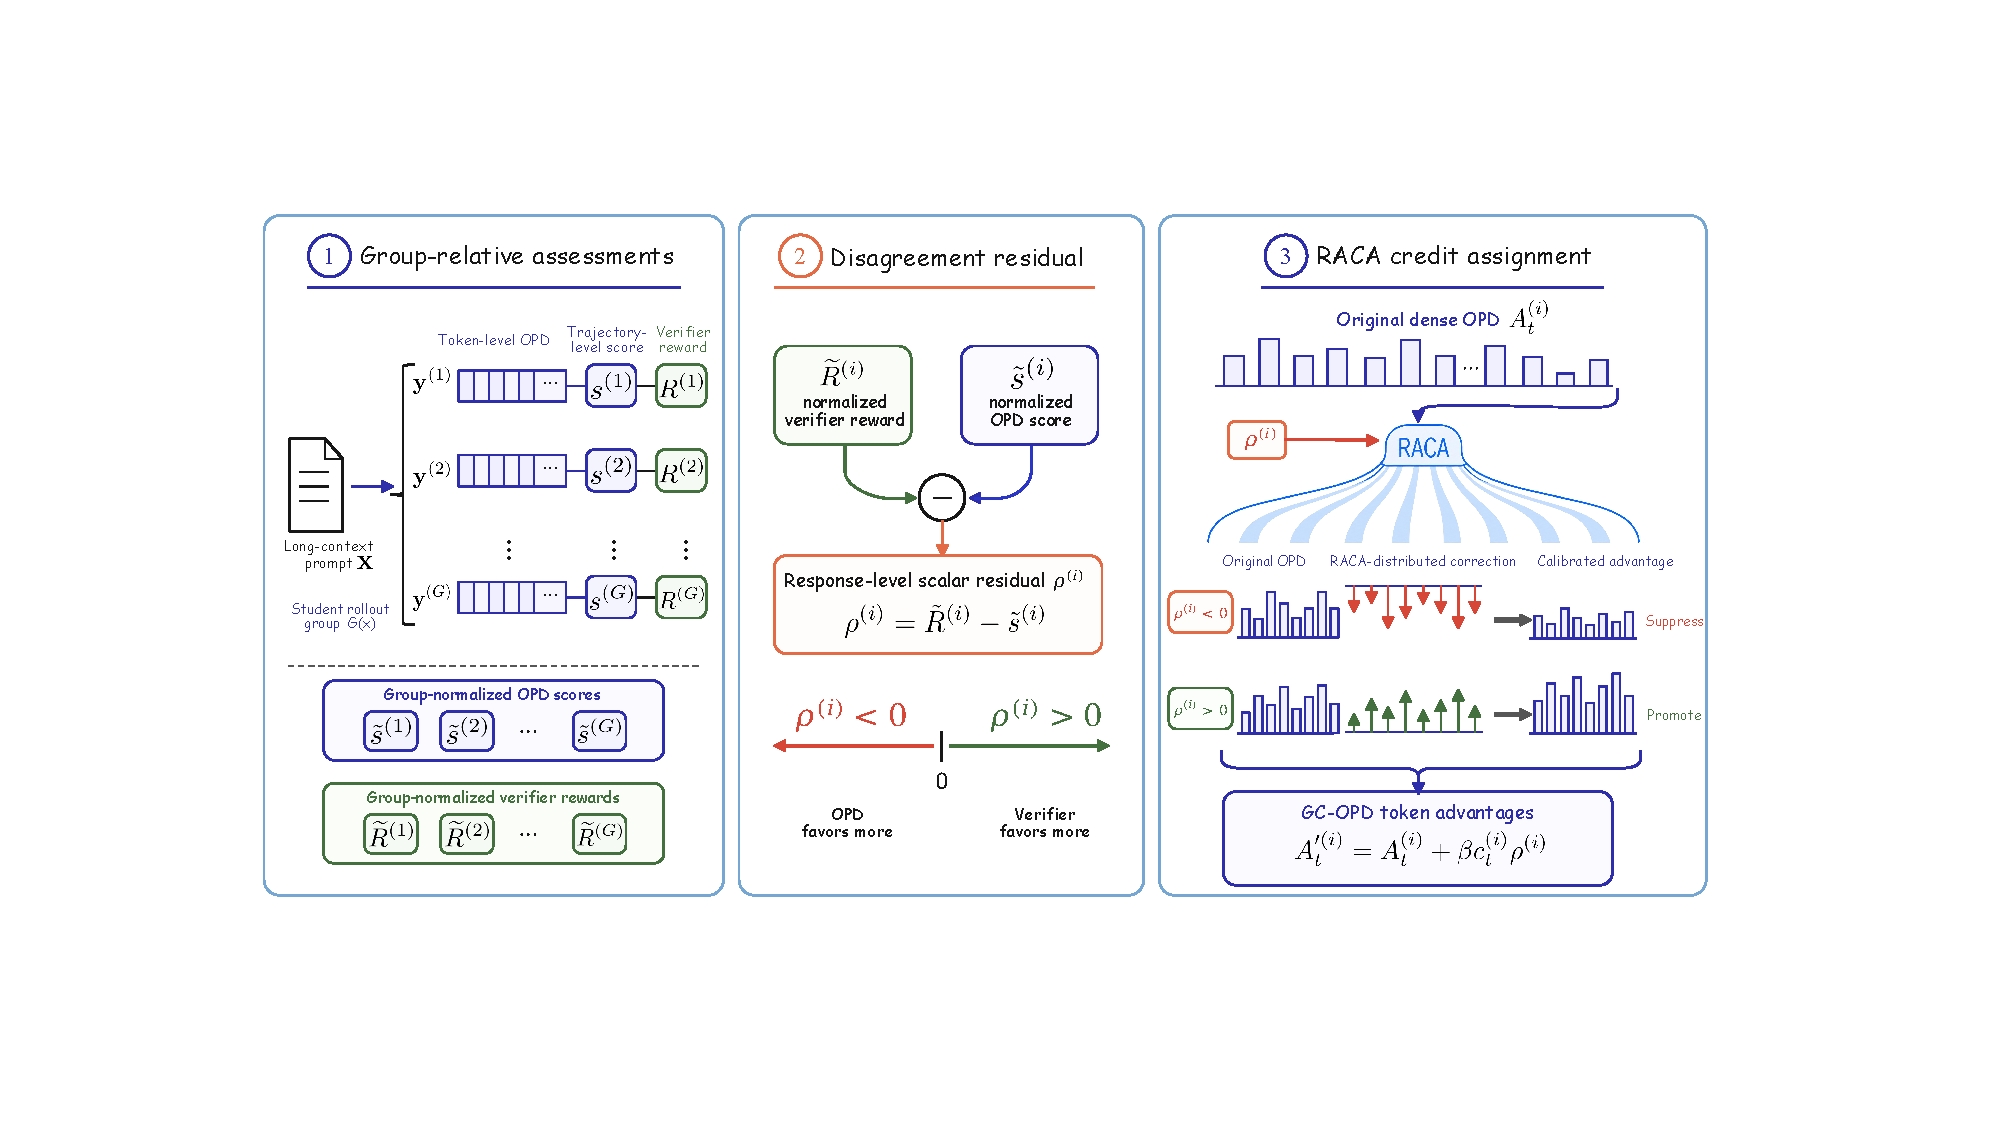
\includegraphics[width=\textwidth]{Figures/gcopd_method/gcopd_method_overview.pdf}
\caption{Overview of \method{}. GC-OPD computes group-normalized verifier rewards and trajectory-level OPD scores, forms their signed residual, and uses RACA to distribute the residual across response tokens while retaining the original OPD advantage.}
\label{fig:gcopd-overview}
\end{figure}
\else
\begin{figure*}[t]
\centering
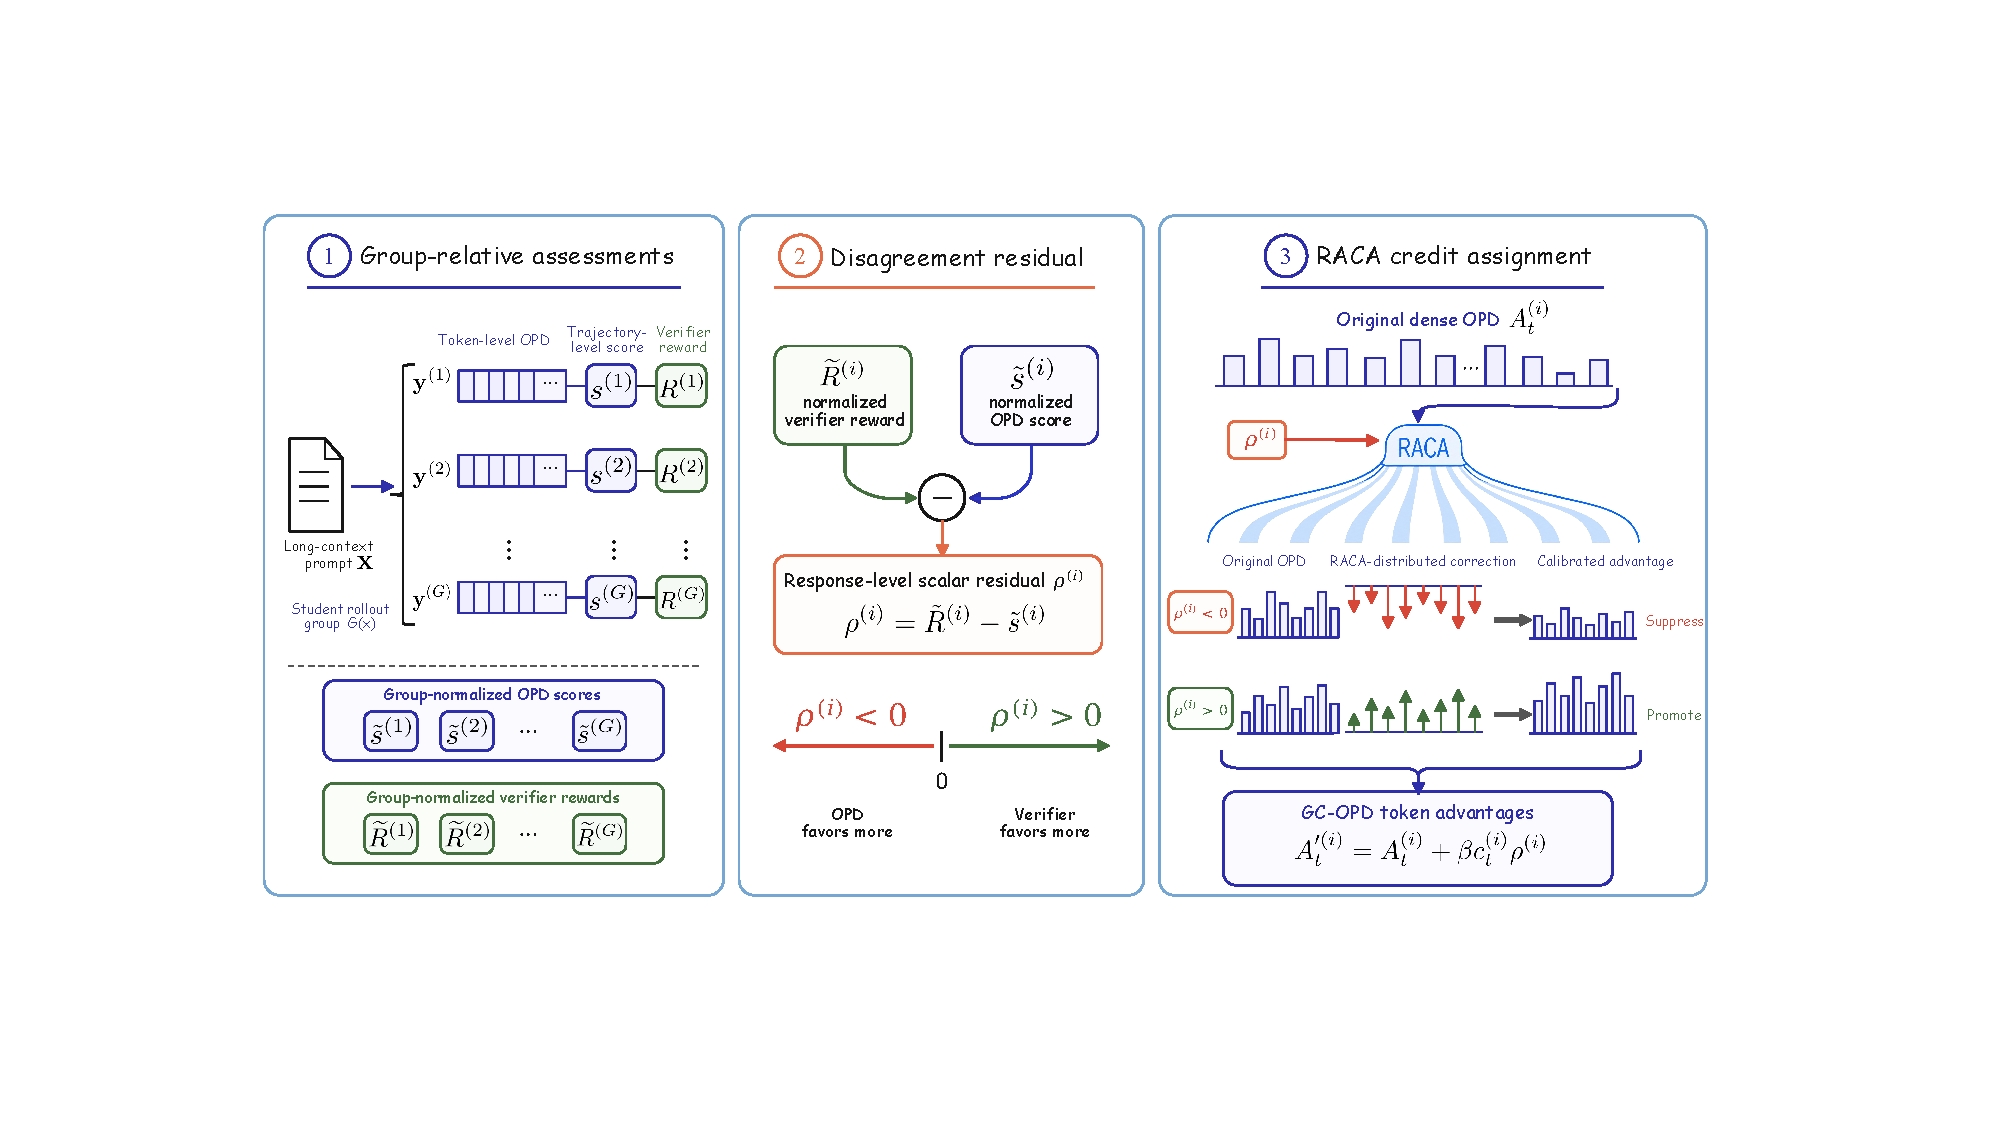
\includegraphics[width=\textwidth]{Figures/gcopd_method/gcopd_method_overview.pdf}
\caption{Overview of \method{}. GC-OPD computes group-normalized verifier rewards and trajectory-level OPD scores, forms their signed residual, and uses RACA to distribute the residual across response tokens while retaining the original OPD advantage.}
\label{fig:gcopd-overview}
\end{figure*}
\fi
